\documentclass{article}

\usepackage{graphicx}
\usepackage{tikz}
\usepackage{tikzsymbols}
\usetikzlibrary{calc,patterns,shapes.geometric}
\pagestyle{empty}
\usepackage[margin=0pt]{geometry}
\geometry{papersize={14in,12in}}

\def\centerarc[#1](#2)(#3:#4:#5){\draw[#1] ($(#2)+({#5*cos(#3)},{#5*sin(#3)})$) arc (#3:#4:#5);}

\begin{document}
	\begin{figure}
		\centering
		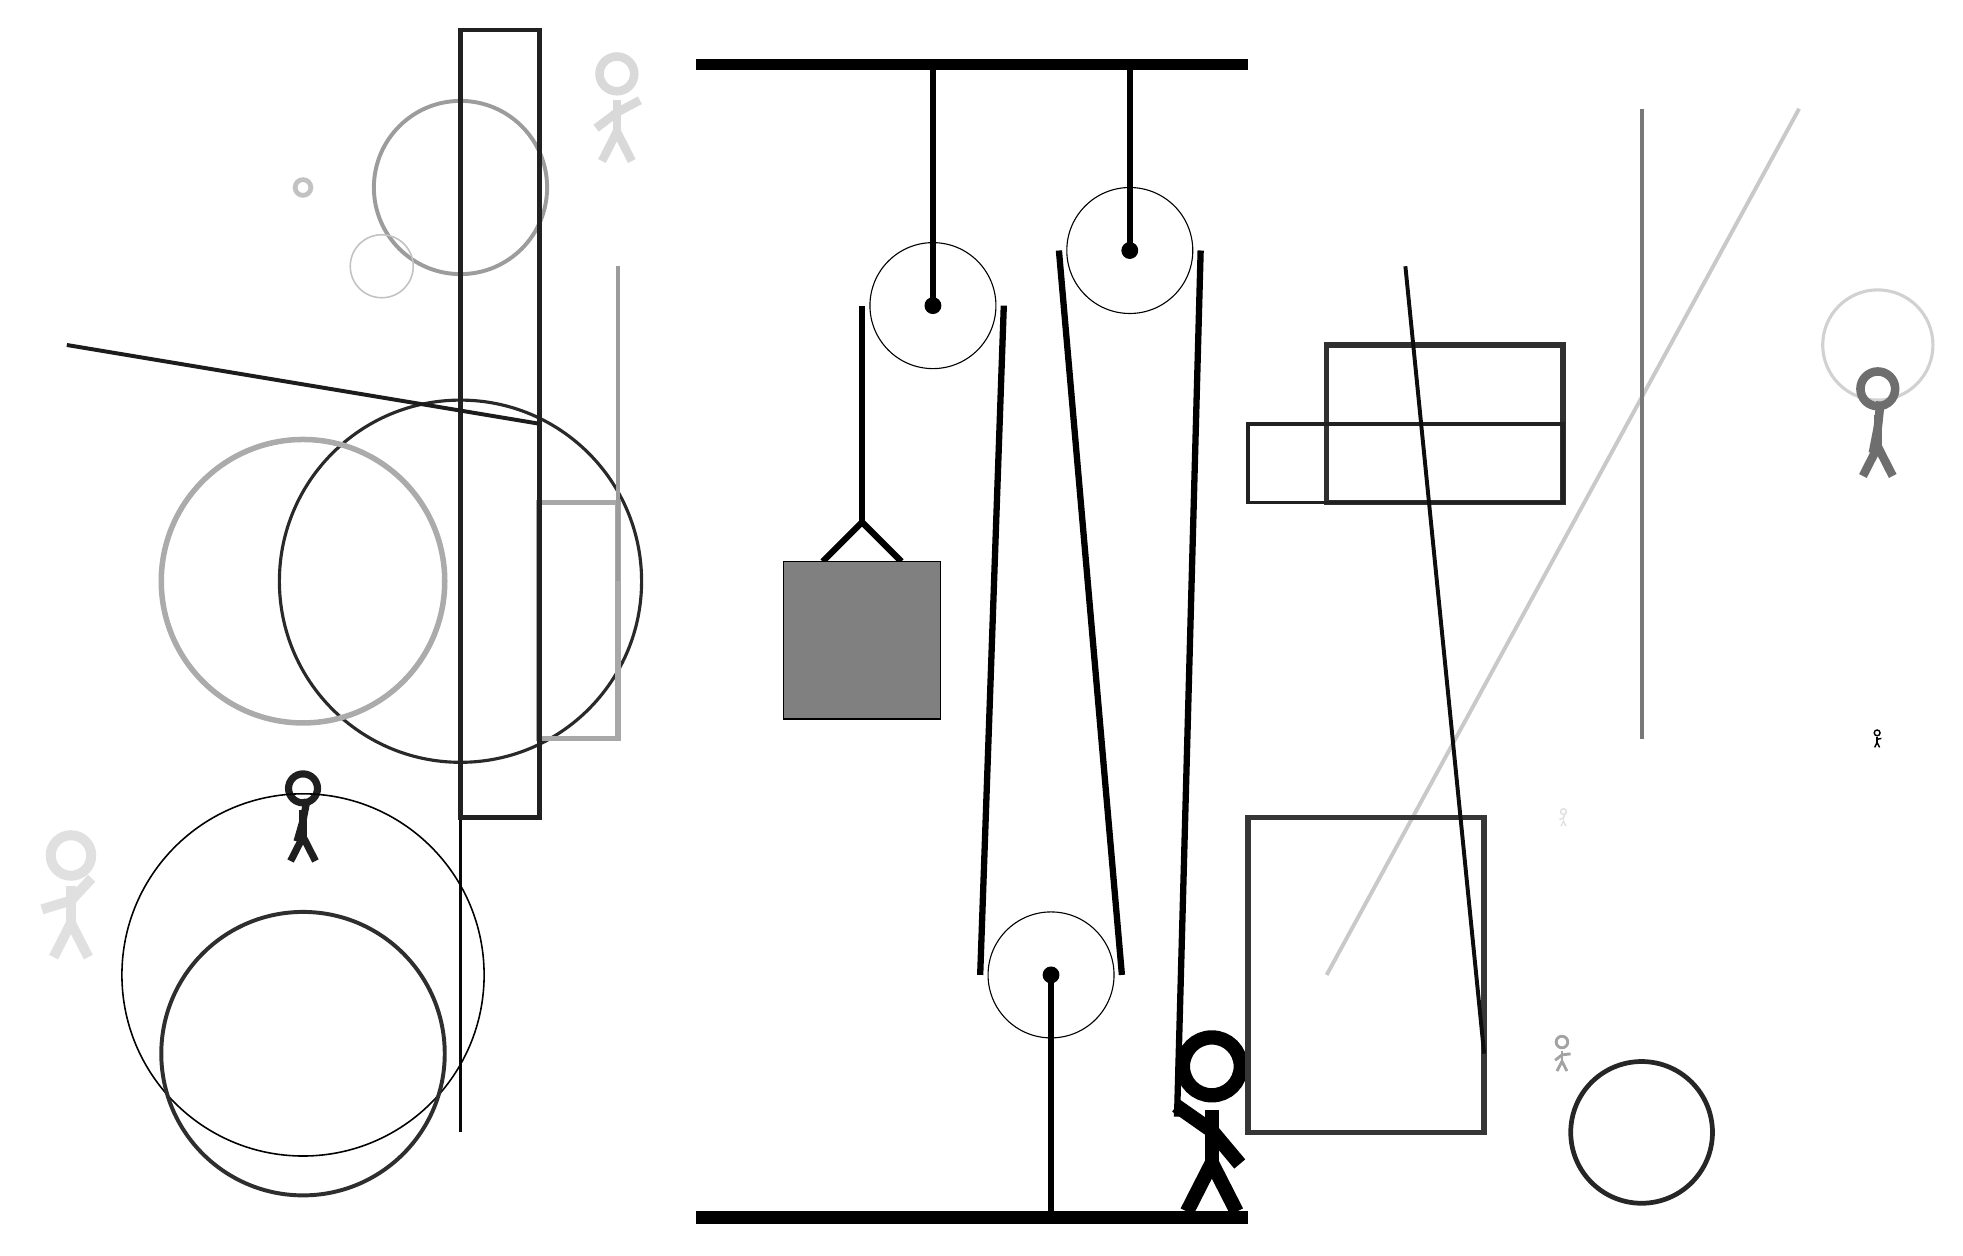
\begin{tikzpicture}
			%%%%% START %%%%%
			
			\draw[fill=black] (-2, 11.5) rectangle (5, 11.625);
			
			\draw (1, 8.5) circle (0.8);
			\draw[fill=black] (1, 8.5) circle (0.1);
			\draw[line width=0.8mm]  (1, 11.5) -- (1, 8.5);
			
			\draw[fill=white](2.5, 0.0) circle (0.8);
			\draw[fill=black] (2.5, 0.0) circle (0.1);
			\draw[line width=0.8mm]  (2.5, -3) -- (2.5, 0.0);
			
			\draw[fill=white](3.5, 9.2) circle (0.8);
			\draw[fill=black] (3.5, 9.2) circle (0.1);
			\draw[line width=0.8mm] (3.5, 11.5) -- (3.5, 9.2);
			
			\draw[line width=0.8mm] (-0.4, 5.25) -- (0.1, 5.75) -- (0.6, 5.25);
			\draw[fill=black!50] (-0.9, 5.25) rectangle (1.1, 3.25);
			
			\draw[line width=0.8mm] (0.1, 8.5) -- (0.1, 5.75);
			\centerarc[line width=0.8mm](1, 8.5)(0:180:0.9);
			\draw[line width=0.8mm](1.9, 8.5) -- (1.6, 0.0);
			\centerarc[line width=0.8mm](2.5, 0.0)(180:360:0.9);
			\draw[line width=0.8mm](3.4, 0.0) -- (2.6, 9.2);
			\centerarc[line width=0.8mm](3.5, 9.2)(0:180:0.9);
			\draw[line width=0.8mm](4.4, 9.2) -- (4.1, -1.8);
			
			\node at (4.5, -1.9) {\Strichmaxerl[10][-35][-50]};
			
			\node[line width=0.5mm, color=black!88] at (-7, 2) {\Strichmaxerl[5][74][79]};
			
			\draw [line width=0.5mm, color=black!39](-5, 10) circle (1.1);
			\draw [line width=0.4mm, color=black!84](-5, 5) circle (2.3);
			\draw[line width=0.5mm, color=black!40] (7, 3) rectangle (7, 3);
			
			\draw[line width=0.7mm, color=black!81] (6, 6) rectangle (9, 8);
			\draw [line width=0.2mm, color=black!24](-6, 9) circle (0.4);
			
			\draw[line width=0.5mm, color=black!97](-5, 7) -- (-5, -2);
			\draw[line width=0.5mm, color=black!21](6, 0) -- (12, 11);
			\node[line width=0.4mm, color=black!12] at (9, 2) {\Strichmaxerl[1][19][72]};
			\draw[line width=0.7mm, color=black!34] (-3, 6) rectangle (-4, 3);
			
			\node[line width=0.7mm, color=black!12] at (-10, 1) {\Strichmaxerl[7][17][47]};
			\draw[line width=0.6mm, color=black!87] (-4, 2) rectangle (-5, 12);
			\node[line width=0.7mm, color=black!15] at (-3, 11) {\Strichmaxerl[6][37][28]};
			
			\draw[line width=0.7mm, color=black!79] (5, -2) rectangle (8, 2);
			\node[line width=0.4mm, color=black!100] at (13, 3) {\Strichmaxerl[1][82][12]};
			\draw [line width=0.2mm, color=black!100](-7, 0) circle (2.3);
			
			\draw [line width=0.5mm, color=black!82](-7, -1) circle (1.8);
			\node[line width=0.5mm, color=black!36] at (9, -1) {\Strichmaxerl[2][38][7]};
			\draw[line width=0.5mm, color=black!89](-4, 7) -- (-10, 8);
			\draw [line width=0.4mm, color=black!18](13, 8) circle (0.7);
			\draw[line width=0.5mm, color=black!53](10, 3) -- (10, 11);
			
			\draw [line width=0.6mm, color=black!24](-7, 10) circle (0.1);
			
			\draw [line width=0.6mm, color=black!85](10, -2) circle (0.9);
			\draw[line width=0.5mm, color=black!87] (5, 7) rectangle (9, 6);
			\node[line width=0.6mm, color=black!57] at (13, 7) {\Strichmaxerl[6][79][84]};
			
			\draw [line width=0.7mm, color=black!33](-7, 5) circle (1.8);
			
			\draw[line width=0.5mm, color=black!95](7, 9) -- (8, -1);
			\draw[line width=0.5mm, color=black!39](-3, 9) -- (-3, 5);
			
			\draw[fill=black] (-2, -3) rectangle (5, -3.15);
			
			%%%%% END %%%%%
		\end{tikzpicture}
	\end{figure}	
\end{document}